\newpage

\section{Grundlagen}

In diesem Kapitel werden die theoretischen und technischen Grundlagen dieser Arbeit erläutert. Zunächst wird ein Überblick über neuronale Netze gegeben, wobei ihr Aufbau, verschiedene Architekturen sowie das Training mittels Backpropagation und Gradient Descent beschrieben werden. Anschließend folgt eine Einführung in analoge Computer, ihre historische Entwicklung sowie ihre typischen Komponenten und Bauweisen. Schließlich werden energiebasierte Modelle behandelt, mit einem besonderen Fokus auf das Hopfield-Netzwerk und das Equilibrium Propagation, deren mathematische Grundlagen und theoretische Anwendung für diese Arbeit von zentraler Bedeutung sind.

\subsection{Neuronale Netze}

\subsubsection{Aufbau und Arten neuronaler Netze}

\begin{quote}
  "`Birds inspired us to fly, burdock plants inspired Velcro, and nature has in- spired countless more inventions. It seems only logical then, to look at the brain’s architecture for inspiration on how to build an intelligent machine"' (\cite[S. 279]{Geron2019})
\end{quote}

Neuronale Netze wurden erstmals 1943 von den Wissenschaftlern Warren S. McCulloch und Walter Pitts in ihrer gemeinsamen Arbeit „A logical calculus of the ideas immanent in nervous activity“ \cite{McCulloch1943} eingeführt. Sie stellten ein vereinfachtes Modell eines künstlichen Neurons vor, das lediglich aus binären Eingaben und einer binären Ausgabe besteht und seine Ausgabe aktiviert, sobald sich eine bestimmte Anzahl an Eingabewerten aktiviert. McCulloch und Pitts zeigten, dass dieser einfache Baustein ausreicht, um jeden möglichen logischen Ausdruck als neuronales Netz darzustellen.

Neuronale Netze zeichnen sich mittlerweile durch ihre Vielseitigkeit, Leistungsfähigkeit und Skalierbarkeit aus und haben damit maßgeblich zur Gründung eines neuen Forschungsfeldes, dem „Deep Learning“, beigetragen. \cite{Geron2019} Die neu gewonnen Aufmerksamkeit im Zusammenhang mit Deep Learning brachte Innovationen wie das von OpenAI entwickelte Sprachmodell „GPT-4“ oder der Bildgenerierungs-KI „Midjourney“ hervor, wodurch bewiesen wurde, dass neuronale Netze zur Lösung komplexer Aufgaben geeignet sind und sogar teilweise ähnlich brauchbare Ergebnisse wie ein Mensch liefern können. \cite{OpenAI2024}

Eines der einfachsten neuronalen Netze ist das von \cite{Rosenblatt1958} vorgestellte Perceptron, dieses basiert auf dem Konzept der \ac{tlu}. Die Eingabe- und Ausgabewerte einer \ac{tlu} sind numerisch und den eingehenden Verbindungen ist jeweils eine Gewichtung zugewiesen. Die \ac{tlu} berechnet nun die gewichtete Summe der Eingabewerte \(z=w_1x_1+w_2x_2 ... +w_nx_n=xtw\). Unter Anwendung einer Aktivierungsfunktion \(hw(x)=step(z)\) kann nun berechnet werden, ob die \ac{tlu} den Wert 0 oder 1 ausgibt. Eine Aktivierungsfunktion für diese Art der Neuronen ist i. d. R. eine Heaviside-Funktion oder eine Vorzeichen-Funktion. \cite[vgl. S. 284 ff.]{Geron2019}

Aktivierungsfunktionen aus Buch einfügen

Abbildung aus Buch nachstellen

Eine alleinstehende \ac{tlu} kann ausschließlich für lineare binäre Klassifikation genutzt werden, es berechnet eine gewichtete Summe anhand der Eingabewerte und gibt einen positiven oder negativen Ausgabewert, abhängig von der Überschreitung eines Schwellenwertes. Ein Perceptron stellt nun eine Sammlung dieser Einheiten auf einer einzelnen Ebene dar, wobei jede \ac{tlu} mit jeder Eingabe verbunden ist. Dies wird als Dense Layer oder Fully Connected Layer bezeichnet. Die Eingabewerte des Perceptron werden durch Eingabe-Neuronen geschleust, wozu zusätzlich ein Bias-Neuron gezählt wird. Dieses Neuron gibt konstant den Wert 1 aus und dient dazu, jedem Neuron des Perceptron eine Bias-Gewichtung zuzuweisen. Die Ausgabe eines Perceptron berechnet sich durch \(h_W,b(X)=\rho(XW+b)\) \cite[vgl. S. 284 ff.]{Geron2019}

Das Perceptron kann nun in mehreren Ebenen genutzt werden, um ein \ac{mlp} zu erzeugen. Dieses besteht aus einer Eingabe-Ebene, mindestens einer versteckten Ebene und einer Ausgabe-Ebene. Jede dieser Ebenen ist im \ac{mlp} mit der jeweils nächsten Ebene vollständig verbunden. Das \ac{mlp} kann durch die vorwärts gerichteten Verbindungen auch als \ac{fnn} bezeichnet werden, eines mit vielen versteckten Ebenen wird \ac{dnn} genannt. \cite[vgl. S. 284 ff.]{Geron2019}

Das bisher beschriebene \ac{mlp} kann zur Klassifikation genutzt werden. Um dieses auch auf Regressionen anwenden zu können, muss die Aktivierungsfunktion entweder entfernt oder durch z.B. ReLU ausgetauscht werden, damit die Ausgabeneuronen willkürliche Werte annehmen können. Die Anzahl der Ausgabe-Neuronen muss in dem Fall angepasst werden, sodass jeder geforderte Ausgabewert durch ein Neuron abgebildet ist. \cite[vgl. S. 292 ff.]{Geron2019}

Eine weitere Art des neuronalen Netz ist das \ac{cnn}, dessen Hauptbestandteil die Convolutional-Ebenen sind. Diese Ebenen sind nur jeweils mit einem Ausschnitt der vorherigen Ebene verbunden, wodurch das daraus entstehende neuronale Netz abstrakte Eigenschaften der Eingabe-Neuronen erlernen kann. Da die einzelnen Ebenen hier nicht, wie beim \ac{mlp}, vollständig verbunden sind, erlaubt ein \ac{cnn} eine große Anzahl an Neuronen pro Ebene, ohne den Rechenaufwand für Training und Inferenz exponentiell zu steigern. Durch diese Eigenschaften eignet sich das \ac{cnn} besonders für die Bildbearbeitung, da hier als Eingabe die Pixel genutzt und darin Eigenschaften des Bildes gefunden werden können. \cite[vgl. S. 447 f.]{Geron2019}

Das \ac{rnn} ähnelt vom Aufbau dem \ac{fnn} unterscheidet sich aber durch rückwärts gerichtete Verbindungen. Die Ausgabe eines Neuron wird damit Teil seiner Eingabe, womit es sich Informationen "`merken"' kann. Ein \ac{rnn} kann als Sequenz-zu-Sequenz Netzwerk genutzt werden, es erhält also eine Sequenz an Eingabe-Werten und produziert eine Sequenz an Ausgabe-Werten. Genauso kann jeder Ausgabewert bis auf den letzten ignoriert werden, was als Sequenz-zu-Vektor Netzwerk bezeichnet wird. Andersherum kann ein \ac{rnn} auch einen Vektor als Eingabe erhalten und eine Sequenz ausgeben, wodurch z.B. eine Beschreibung für ein Bild generiert werden könnte. Letztlich ist auch ein sog. Encoder-Decoder Modell möglich, wobei ein Sequenz-zu-Vektor Netzwerk zuerst eine Repräsentation der Eingabesequenz erzeugt, und ein Vektor-zu-Sequenz Netzwerk daraufhin eine Ausgabe aus dieser Repräsentation erzeugt. Ein Anwendungsfall dafür sind Sprachanwendungen wie ein Übersetzer, da jedes Wort eines Textes im Vornherein bekannt sein muss, um eine korrekte Ausgabe zu erzeugen. \cite[vgl. S. 497 ff.]{Geron2019}


\subsubsection{Training neuronaler Netze mit Backpropagation und Gradient Descent}

\subsection{Analoge Computer}

\subsubsection{Geschichte zu analogen Computern}

Die Geschichte des analogen Computers reicht bis in die Antike zurück. So wurde im Jahr 1900 der Antikythera-Mechanismus in einem Schiffswrack entdeckt, der aus etwa 100 v. Chr. stammt. Er gilt als eines der komplexesten mechanischen und mathematischen Geräte der Antike und konnte die Bewegungen von Himmelskörpern modellieren sowie Sonnen- und Mondfinsternisse vorhersagen. \cite[vgl. S. 9 f.]{Ulmann2022}

Im Verlauf der technischen Entwicklung wurden Gleitkomma-Rechner konstruiert, mechanische Geräte, die zur Lösung komplexer mathematischer Probleme, wie der Berechnung von Bombenflugbahnen und Feuerleitsystemen, eingesetzt wurden. Diese fanden auch in friedlichen Anwendungen wie der Gezeiten-Berechnung Verwendung. \cite[vgl. S. 9]{Ulmann2022}

Mit dem Fortschritt der Technik entstanden die ersten elektronischen analogen Computer, die von Helmut Hoelzer in Deutschland und George A. Philbrick in den USA entwickelt wurden. Diese Computer wurden primär für militärische Anwendungen wie Flugbahn- und Feuerleitsysteme genutzt. Ein Beispiel für einen frühen elektronische Analogrechner ist Hoelzers Mischgerät, das während des zweiten Weltkriegs in Deutschland entwickelt wurde und Elektrohnenröhren zur Durchführung von Berechnungen verwendete. \cite[vgl. S. 41 f.]{Ulmann2022}

Ein weiteres bedeutendes Gerät war der Caltech-Computer, ein elektronischer Analogrechner, der zwischen 1946 und 1947 entwickelt wurde und etwa 15 Tonnen wog. Dieser Computer wurde zur Lösung komplexer mathematischer und wissenschaftlicher Probleme, einschließlich Differentialgleichungen, entwickelt. \cite[vgl. S. 69]{Ulmann2022}

George A. Philbrick spielte eine bedeutende Rolle in der Weiterentwicklung und Verbreitung elektronischer Analogrechner. Er führte kommerzielle Operationsverstärker ein und entwickelte in den 1950er Jahren modulare elektronische Analogrechner, was einen großen Einfluss auf die Standardisierung und Verbreitung dieser Technologie hatte. \cite[vgl. S. 136]{Ulmann2022}


\subsubsection{Typische Komponenten und Bauweisen analoger Computer}
\label{chap:Typische Komponenten und Bauweisen analoger Computer}

Der Operationsverstärker gilt als zentraler Baustein für die meisten Komponenten eines analogen Rechners. Er bildet die Differenz aus zwei Eingangssignalen und verstärkt dieses Signal anschließend. Werden ein freies und ein geerdetes Eingangssignal genutzt, so wird nur das Freie verstärkt. Durch ein Rückkopplungs-Signal gelingt es dem Operationsverstärker einen Teil der Stromverstärkung aufzugeben, um Stabilität zu gewinnen. Dieses Signal verbindet die Ausgabe der Komponente mit seiner Eingabe, wobei diese beiden Werte miteinander summiert werden. Ein wichtiges Merkmal dieser Komponente ist außerdem, dass das Vorzeichen der Eingabe gedreht wird. \cite[vgl. S. 73 f.]{Ulmann2022}

\begin{figure}[h]
  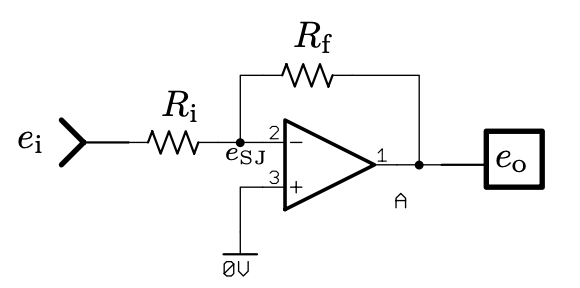
\includegraphics[width=0.5\textwidth]{abbildungen/opamp_mit_rueckkopplung.png}
  \caption{Operationsverstärker mit Rückkopplung. Quelle: \cite[S. 76]{Ulmann2022}}
  \label{fig:Operationsverstärker mit Rückkopplung}
\end{figure}

Die Formel zu Berechnung der Ausgangsspannung lautet damit wie folgt:

\[e_o=\frac{R_f}{R_i}e_i\]

Durch Anpassungen des Eingangssignals bzw. des Rückkopplungs-Signals kann die Funktion des Operationsverstärkers geändert werden. So sind hiermit Operationen wie Summieren, Subtrahieren, Invertieren, das Multiplizieren von Konstanten, Integration und (bedingt) die Differenzierung möglich.

Im Prozess der Verstärkung der Signale kann ein sog. Drift auftreten. Dadurch werden kleine Fehler in der Signalverarbeitung verstärkt und führen zu großen Fehlern am Ausgang. Dieses Problem kann durch Drift-Stabilisierung gelöst werden, wie beschrieben in einem Patent von \cite{Goldberg1954}. Das durch Drift verursachte Fehlersignal kann an der Summe des Eingangs- und Rückkopplungs-Signals ausgelesen werden. Es wird verstärkt und als weiteres Eingangssignal genutzt. Somit wird der Drift ausgeglichen. \cite[vgl. S. 80]{Ulmann2022}

Um einen Summierer zu bilden, muss lediglich ein weiteres Eingangssignal zum Operationsverstärker hinzugefügt werden. Die Widerstände \(R_i\) bilden die Koeffizienten der Eingangssignale. Der Summierer bildet also die gewichtete Summe der Eingangssignale und gibt diese invertiert aus. \cite[vgl. S. 86]{Ulmann2022}

Wird der Feedback-Widerstand \(R_f\) durch einen Kondensator \(C\) ersetzt, wird die Summe der Eingangssignale über Zeit integriert. Man erhält also einen Integrierer. Durch ein Steuerelement \textit{IC} wird ein Initialwert festgelegt, der so lange ausgegeben wird, bis ein weiteres Steuerelement \textit{OP} betätigt wird. Im aktivierten Zustand wird so lange das Integral der Eingangssignale ausgegeben, bis der \textit{OP} Schalter erneut betätigt und der letzte gespeicherte Wert ausgegeben wird. \cite[vgl. S. 89 ff.]{Ulmann2022}

Die Anwendung eines Koeffizienten am Operationsverstärker kann durch ein Potentiometer erfolgen, welches am Eingangssignal angeschlossen ist. Das somit erhaltene Koeffizient-Potentiometer lässt sich über einen speziellen Zustand des Analogrechners, dem \textit{Potentiometer Set} (kurz: \textit{Pot Set}) setzen. In diesem Zustand werden alle Recheneinheiten des Analogrechners deaktiviert, sodass das rohe Eingangssignal weitergeleitet wird. In großen analogen Rechnern werden Potentiometer durch Servomotoren oder in hybriden Rechnern digital gesteuert. \cite[vgl. S. 92 ff.]{Ulmann2022}

Ein Funktionsgenerator kann genutzt werden, um eine beliebige Funktion \(f(x,...)\) abzubilden. Für analoge Rechner ist das aber eine komplexe Aufgabe, weshalb sich für diesen Anwendungsfall hybride Systeme besonders eignen. Als mögliche analoge Ansätze bieten sich der servogetriebene Funktionsgenerator, der Kurvenfolger oder der Fotoformer an \cite[vgl. S. 97 ff.]{Ulmann2022}.

\begin{figure}[h]
  \centering
  \begin{subfigure}[b]{0.2\textwidth}
    
\includegraphics[width=\textwidth]{abbildungen/symbol_summierer.png}
    \caption{Summierer}
  \end{subfigure}%
  \hfill
  \begin{subfigure}[b]{0.2\textwidth}
    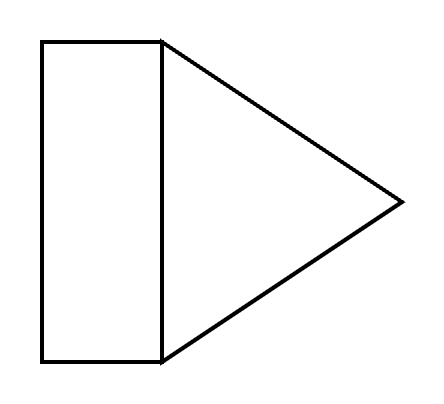
\includegraphics[width=\textwidth]{abbildungen/symbol_integrierer.png}
    \caption{Integrierer}
  \end{subfigure}%
  \hfill
  \begin{subfigure}[b]{0.2\textwidth}
    
\includegraphics[width=\textwidth]{abbildungen/symbol_potentiometer.png}
    \caption{Potentiometer}
  \end{subfigure}%
  \hfill
  \begin{subfigure}[b]{0.2\textwidth}
    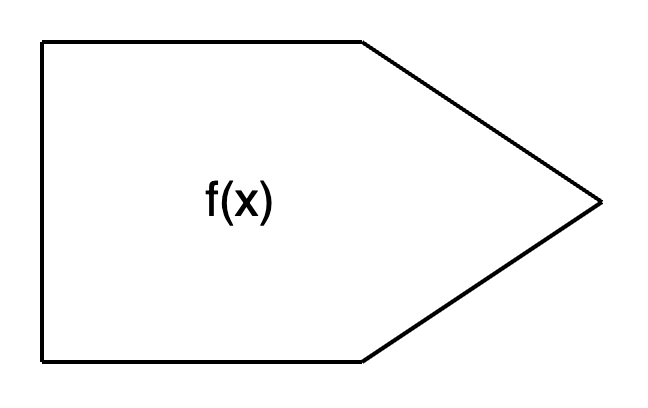
\includegraphics[width=\textwidth]{abbildungen/symbol_funktionsgenerator.png}
    \caption{Funktionsgenerator}
  \end{subfigure}
  \caption{Symbole zur Darstellung eines analogen Computers. Quelle: \textit{Eigene Darstellung}}
  \label{fig:Symbole analoger Computer}
\end{figure}

Die im ersten Augenblick einfache Multiplizierung ist auf analogen Rechnern komplex zu implementieren \cite[vgl. S. 105]{Ulmann2022}. Moderne analoge Rechner greifen typischerweise auf die Gilbert Zelle zurück. Die Berechnung einer Division bzw. Quadratwurzel kann durch modifizierte Multiplikatoren erfolgen. \cite[S. 114 f.]{Ulmann2022}

Ein Komparator kann \zb zur Implementierung einer Schrittfunktion oder zum Tauschen von Variablen genutzt werden. Um das zu erreichen, reicht es schon aus, Dioden in der Feedback-Schleife eines Operationsverstärkers zu platzieren. Nach einem ähnlichen Prinzip kann auch ein Begrenzer erzeugt werden, dessen Eingangssignal zwischen einer Ober- und Untergrenze limitiert wird. \cite[S. 116]{Ulmann2022}

Die im Jahr 2020 gegründete anabrid GmbH hat es sich zum Ziel gesetzt, analoge und digitale Technologien zu kombinieren, um die technologischen Herausforderungen der Zukunft effizient lösen zu können. Dazu entwickelt und vertreibt das Unternehmen rekonfigurierbare analoge Rechner, wie den 2024 erschienenen "`lucidac"' oder das rudimentäre "`The Analog Thing"' \cite{AnabridWebsite}.

\begin{quote}
  "`THE ANALOG THING is a high-quality, low-cost, open-source, and not-for-profit cutting-edge analog computer. You can think of it as a kind of Raspberry Pi that computes with continuous voltages rather than with zeroes and ones."' (\cite{TheAnalogThingDocs})
\end{quote}

Das \ac{that} orientiert sich am historischen Design der analogen Computer und arbeitet demnach mit Patchkabeln, mit denen Rechenelemente verschaltet werden (siehe Abbildung \ref{fig:The Analog Thing}). Dabei arbeitet das Gerät mit 10 Volt und in einem Wertebereich von \pm 1. Fällt eine Spannung außerhalb dieses Wertebereichs, fällt das Gerät in den sog. "`Overload"'-Modus und signalisiert dies über eine LED. Außerdem bietet das Gerät Anschlüsse für einige Variablen, welche als Ein- oder Ausgaben zur Auswertung oder Verschaltung mit weiteren analogen Rechnern genutzt werden können \cite{TheAnalogThingDocs}.

\begin{figure}[h]
  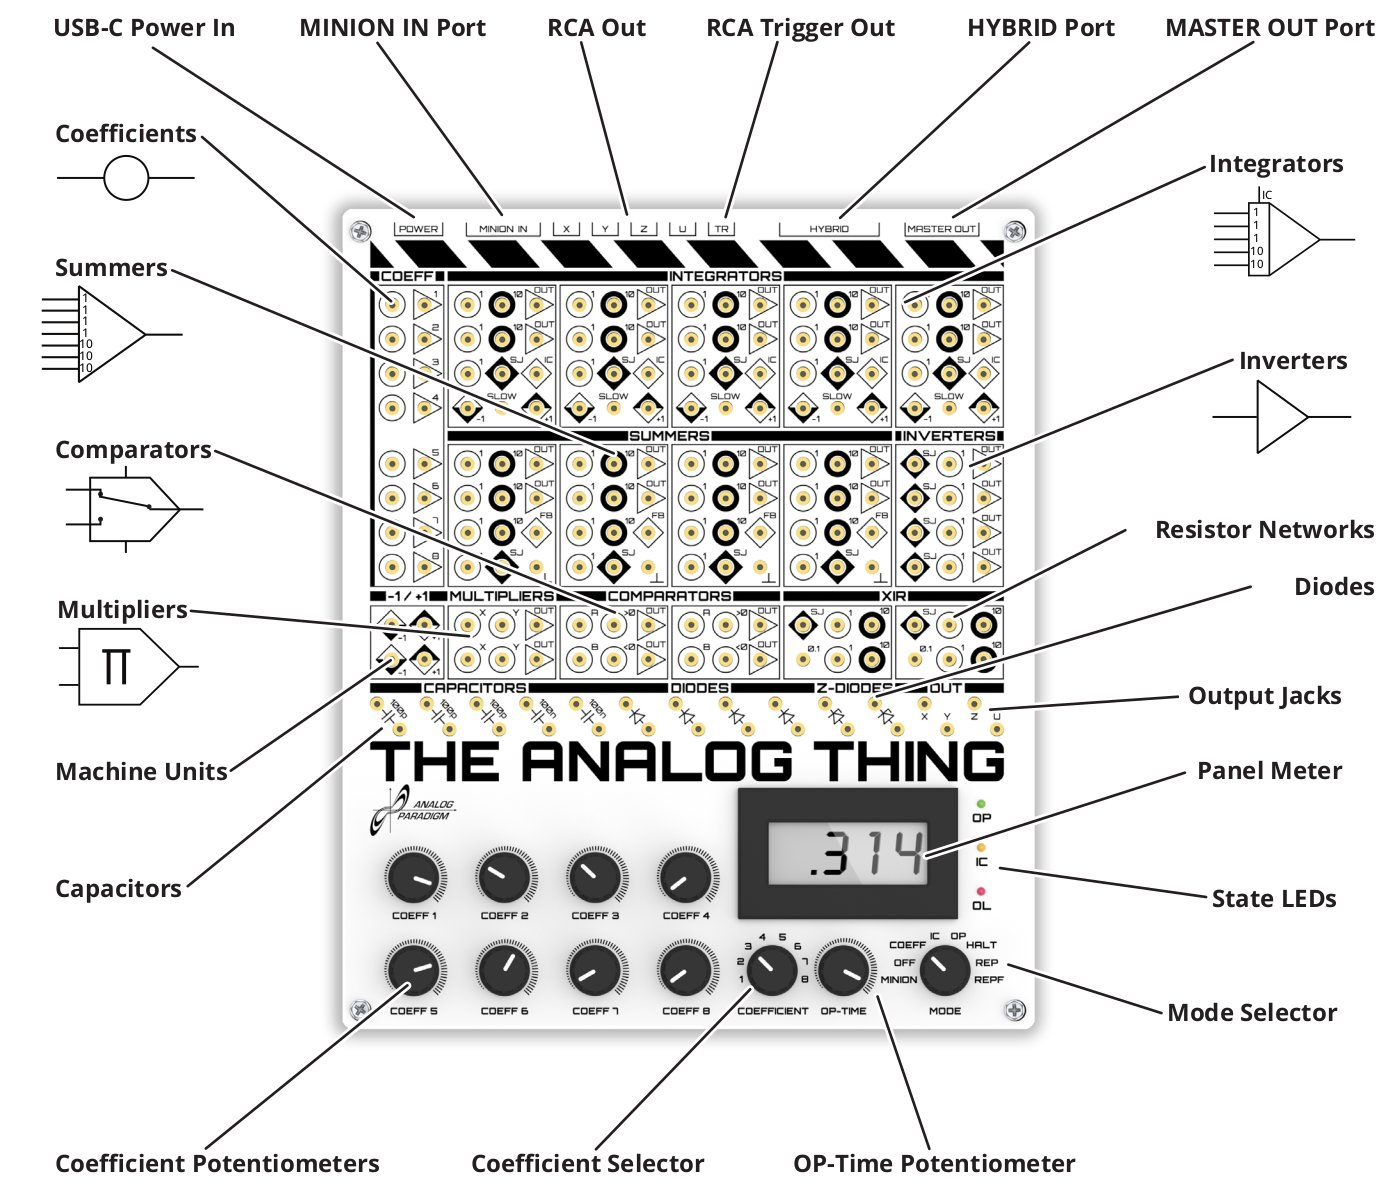
\includegraphics[width=0.75\textwidth]{abbildungen/the_analog_thing.jpg}
  \caption{The Analog Thing des Herstellers anabrid GmbH. Quelle: \cite{TheAnalogThingDocs}}
  \label{fig:The Analog Thing}
\end{figure}

Wie in Abbildung \ref{fig:The Analog Thing} zu sehen, bietet das \ac{that} die grundlegenden Komponenten wie Potentiometer, Summierer, Integrierer, Multiplizierer und Komparatoren an. Diese Komponenten reichen bereits aus, um Probleme wie die Euler-Spirale zu lösen (Siehe Abbildung \ref{fig:THAT Euler Spirale})

\begin{figure}[h]
  \begin{subfigure}{.2\textwidth}
    \centering
    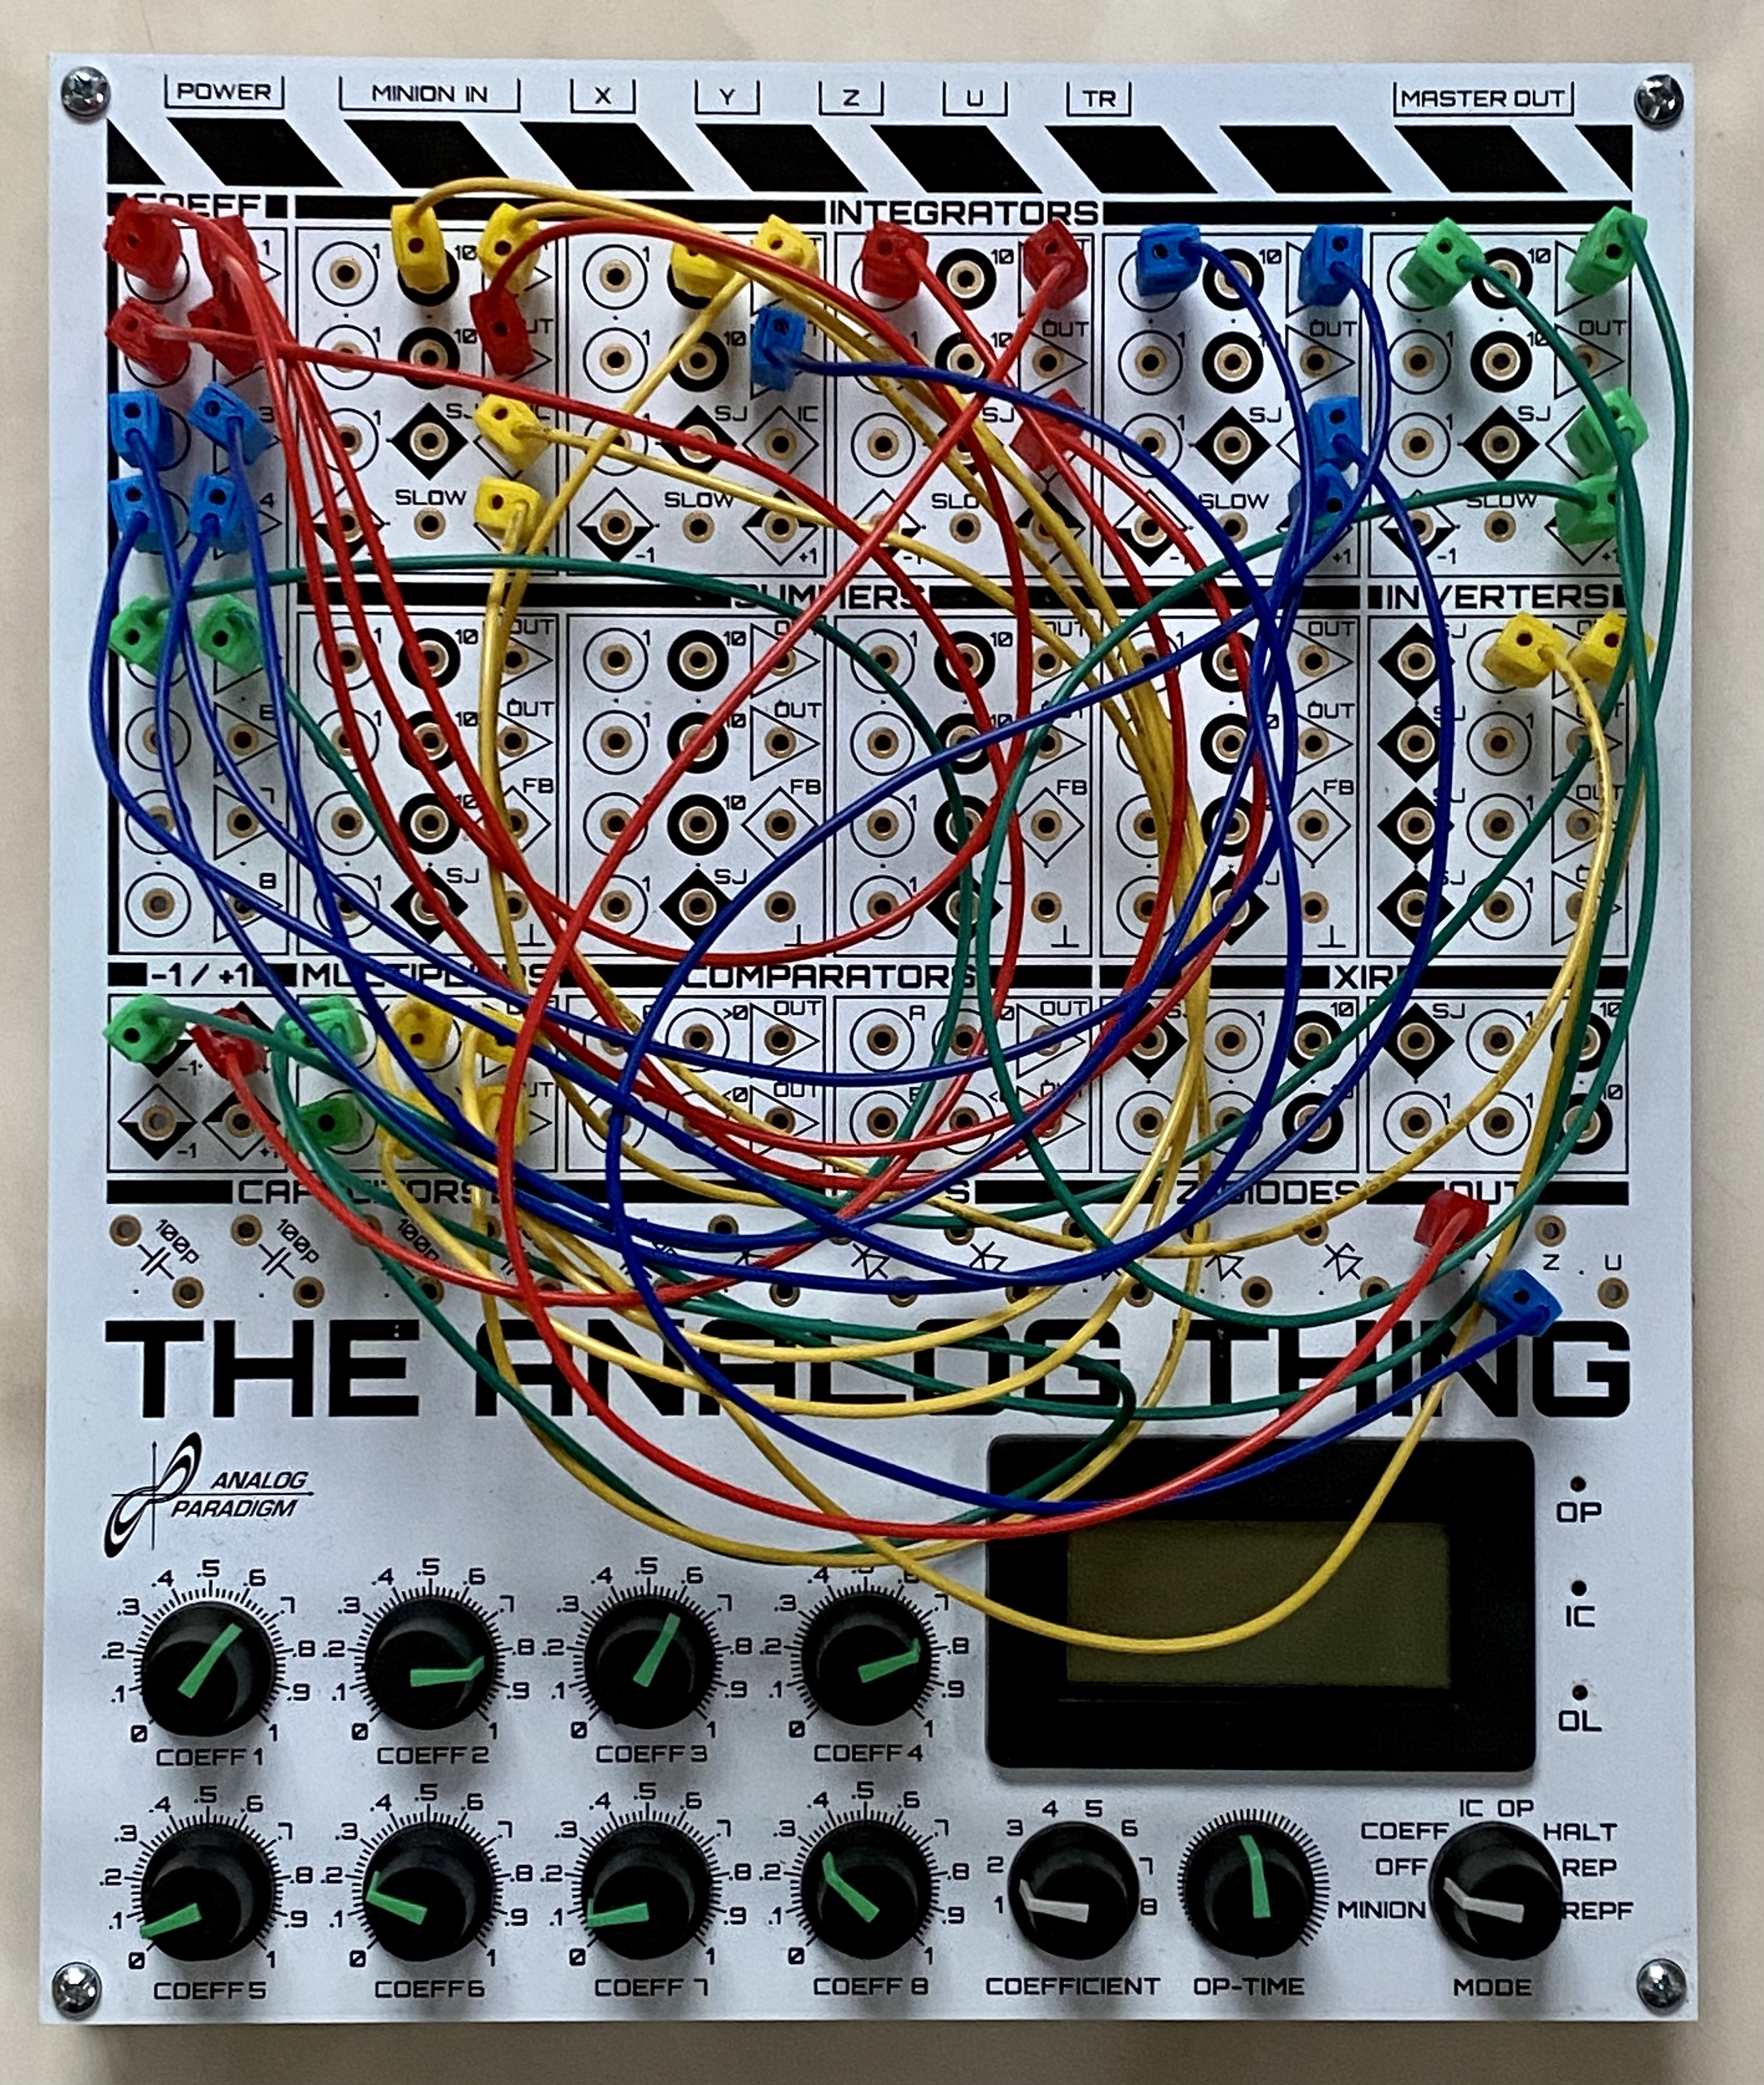
\includegraphics[width=\textwidth]{abbildungen/euler_spirale_implementierung.jpg}\par
  \end{subfigure}
  \begin{subfigure}{.2\textwidth}
    \centering
    
\includegraphics[width=\textwidth]{abbildungen/euler_spirale_ausgabe.jpg}\par
  \end{subfigure}
  \caption{Simulation der Euler-Spirale auf einem \ac{that}. Quelle: \cite{TheAnalogThingDocs}}
  \label{fig:THAT Euler Spirale}
\end{figure}

Das neueste Modell des Herstellers Anabrid, der "`lucidac"', lasst sich digital über Software progammieren, wodurch der manuelle Aufwand durch die Verkabelung des Rechners wegfällt \cite[vgl.]{AnabridLucidAC2025}. Dafür wurde eine Python-Bibliothek entwickelt, die durch Befehle wie "`connect(a, b)"' Verbindungen zwischen Komponenten herstellen kann \cite[vgl.]{AnabridLucipy}. Um die software-gesteuerte Programmierung zu ermöglichen, verwendet der lucidac eine Verbindungs-Matrix, welche der Verbindung aller Komponenten ein Gewicht zuweist. Wird ein Wert innerhalb der Matrix von null auf \zb eins geändert, so wird eine neue (gewichtete) Verbindung hergestellt \cite{AnabridLucidAC2025}. Seien \(C^{in}\) bzw. \(C^{out}\) die Ein- bzw. Ausgaben der Komponenten und \(M\) die gewichteten Verbindung zwischen Komponenten, so gilt:

\[C_i^{in}=\sum_{j=0}^{16}M_{ij}C_j^{out}, i,j\in[0,16]\]


\subsubsection{Aufbau von Schaltkreisen zur Lösung von Differenzialgleichungen}

\subsection{Energiebasierte Modelle}

\subsubsection{Definition: energiebasierte Modelle und energiebasiertes Lernen}

\glspl{ebm} finden im maschinellen Lernen Anwendung und arbeiten mithilfe einer Energiefunktion, welche jeder beliebigen Konfiguration an Variablen eine skalare Energie zuweist. Am Beispiel eines neuronalen Netzes könnten diese Variablen die Eingabe-Variablen, die Parameter- und Versteckten-Variablen sowie die Ausgabe-Variablen sein. Zur Inferenz des Modells werden zunächst die Eingabe-Variablen festgelegt und anschließend ein Minimum der Energiefunktion bestimmt. Wurde ein Minimum gefunden, kann die Ausgabe des Modells anhand der Ausgabe-Variablen ausgelesen werden. Ein \ac{ebm} wird durch Anpassung seiner Energiefunktion trainiert, indem sie kleinere Energien für korrekte Werte und größere Energien für falsche Werte generiert. \cite{Lecun2006} Die ersten vorgestellten \ac{ebm} waren das Hopfield-Netzwerk \cite{Hopfield1984} und die auf dem Hopfield-Netzwerk basierende Boltzmann-Maschine \cite{Ackley1985}.


\subsubsection{Das Hopfield-Netzwerk: Eine Herangehensweise an neuronale Netze}
\label{chap:Das Hopfield-Netzwerk: Eine Herangehensweise an neuronale Netze}

In den frühen 1980er Jahren stellte \citeauthor{Hopfield1982} ein neuronales Netzwerkmodell vor, das als bedeutender Meilenstein in der Erforschung kollektiver Berechnungsfähigkeiten gilt. Ziel dieses Modells war es, die Funktionsweise stark vernetzter neuronaler Systeme zu verstehen und ihre Potenziale für Mustererkennung, fehlerresistente Speicherung und assoziatives Gedächtnis zu untersuchen. Diese Netzwerke dienen auch als Modelle für biologisch inspirierte Rechner, die parallele und robuste Berechnungen ermöglichen sollen \cite[vgl. S. 2554]{Hopfield1982} \cite[vgl. S. 3088]{Hopfield1984}.

Die Netzwerktopologie basiert auf vollständig miteinander verbundenen Neuronen, die durch eine symmetrische Gewichtsmatrix \(T_{ij}\) miteinander verknüpft sind. Diese Symmetrie ist entscheidend, um stabile Zustände zu gewährleisten und chaotisches Verhalten zu vermeiden. Ursprünglich wurden die Neuronen mit binären Zuständen modelliert, bei denen jedes Neuron entweder „aktiv“ (1) oder „inaktiv“ (0) ist, was an das McCulloch-Pitts-Modell angelehnt ist \cite[vgl. S. 2555]{Hopfield1982}. Spätere Arbeiten erweiterten das Modell durch die Einführung von Neuronen mit kontinuierlichen, sigmoidalen Ausgabefunktionen, um die biologischen Realitäten besser abzubilden \cite[vgl. S. 3088]{Hopfield1984}.

Ein zentrales Konzept des \gls{hopfieldnetzwerk} ist die Minimierung einer Energiefunktion \(E\), die den Zustand des Netzwerks beschreibt. Diese Funktion ist so definiert, dass sie durch asynchrone Aktualisierungen der Neuronen monoton abnimmt, bis ein lokales Minimum erreicht ist. Diese Minima entsprechen stabilen Zuständen des Netzwerks, die gespeicherte Erinnerungen repräsentieren. Diese Eigenschaft erlaubt es dem Netzwerk, unvollständige oder verrauschte Eingaben zu vervollständigen, wodurch es robust gegenüber Störungen und Ausfällen einzelner Neuronen ist. Die Fähigkeit, Informationen anhand von Teilinformationen abzurufen, macht das \gls{hopfieldnetzwerk} zu einem echten inhaltsadressierbaren Speicher \cite[vgl. S. 2554 f.]{Hopfield1982}.

Das ursprüngliche Modell mit binären Zuständen ist besonders für digitale Berechnungen geeignet und lässt sich effizient simulieren. Das kontinuierliche Modell mit sigmoidalen Neuronen hingegen berücksichtigt biologische Eigenschaften wie graduelle Reaktionskurven und Verzögerungen durch synaptische Übertragungen. Diese Modelle zeigen, dass dieselben kollektiven Eigenschaften, wie sie im ursprünglichen binären Modell beobachtet wurden, auch in biologisch realistischeren Systemen auftreten können. Dies stärkt die These, dass solche kollektiven Eigenschaften tatsächlich in natürlichen neuronalen Netzwerken vorkommen \cite[vgl. S. 3089]{Hopfield1984}.

Ein weiterer Aspekt ist die Kapazität des Netzwerks, mehrere stabile Zustände oder Erinnerungen gleichzeitig zu speichern. Studien zeigen, dass ein Netzwerk mit \(N\) Neuronen etwa \(0,15N\) stabile Zustände speichern kann, bevor die Fehlerrate signifikant ansteigt. Die Speicherkapazität ist somit begrenzt, kann jedoch durch gezielte Anpassungen der Schwellenwerte und Gewichtungen erhöht werden. Darüber hinaus bietet das Netzwerk eine hohe Fehlertoleranz und kann ähnliche Muster in Kategorien zusammenfassen, was es zu einem effektiven Werkzeug für Mustererkennungsaufgaben macht \cite[vgl. S. 2556]{Hopfield1982} \cite[vgl. S. 3091]{Hopfield1984}.

Das \gls{hopfieldnetzwerk} hat nicht nur Bedeutung für die Neurobiologie, sondern auch für technische Anwendungen. Seine analoge Implementierung in integrierten Schaltkreisen ermöglicht die Entwicklung von robusten, fehlertoleranten Speichern und Prozessoren. Dieses Netzwerk ist insbesondere für parallele Berechnungen und selbstorganisierende Systeme nützlich, was es für Anwendungen im maschinellen Lernen und in autonomen Systemen relevant macht. Durch seine Fähigkeit, kollektive Berechnungen durchzuführen, bietet es eine Grundlage für fortschrittliche Algorithmen in der künstlichen Intelligenz \cite[vgl. S. 2554 ff.]{Hopfield1982}.

Neuere Forschungen untersuchen die Auswirkungen von Asymmetrien in der Gewichtsmatrix und die Einbeziehung von nichtlinearen Dynamiken, um zeitabhängige Sequenzen und komplexere Berechnungen zu ermöglichen. Diese Erweiterungen zeigen, dass das \gls{hopfieldnetzwerk} flexibel genug ist, um als Grundlage für vielfältige Anwendungen zu dienen. Seine Robustheit gegenüber Rauschen und Störungen macht es besonders geeignet für reale Umgebungen, in denen Perfektion selten ist \cite[vgl. S. 2557]{Hopfield1982} \cite[vgl. S. 3092]{Hopfield1984}.


\subsubsection{Energiebasiertes Lernen am Beispiel Equilibrium Propagation}

\paragraph{Mathematische Grundlagen}

\textbf{TODO: Seitenzahlen für Quellenangaben}

Ein Verfahren zum Trainieren \glspl{ebm} stellt das \gls{eqprop} dar. In diesem Verfahren wird der Gradient einer Energiefunktion bestimmt und damit die Parameter des Modells angepasst. Die Vorhersagen des Modells werden aus dem Datenpunkt und den Parametern impliziert anstelle diese explizit zu definieren, weshalb sich dieses Verfahren besonders für die Anwendung auf analogen Computern eignet. \cite{Scellier2017}

Der Zustand des Modells wird durch den Vektor \(s\) dargestellt, \(v\) gibt die Eingabe-Variablen an und \(\theta\) steht für die Parameter des Modells. Die Zustandsvariable \(s\) verändert sich über Zeit, sodass die Energiefunktion \(E(\theta,v,s)\) minimiert wird. Neben der Energiefunktion wird auch eine Kosten-Funktion \(C(\theta,v,s)\) definiert, welche die Diskrepanz zwischen der Ausgabe des Modells und den Zielwerten angibt. Liefert die Energiefunktion für eine Konfiguration an Variablen eine kleinere Energie, so sollte auch der Wert der Kosten-Funktion geringer sein. Zusätzlich wird der Einfluss-Parameter \(\beta\) definiert, der als Skalierungsfaktor für die Kostenfunktion dient. Das Equilibrium Propagation definiert nun eine Gesamtenergiefunktion \(F\) als:

\[F(\theta,v,\beta,s):=E(\theta,v,s)+\beta C(\theta,v,s)\]

Die Fixpunkte des Modells werden in der Form \(s_{(\theta,v)}^\beta\) dargestellt, und stehen für jeweils ein lokales Minimum der Gesamtenergiefunktion \(F\). Mit \(\beta=0\) ergibt sich \(s_{(\theta,v)}^0\), ein Minimum der Energiefunktion \(E\) und damit die Vorhersage des Modells. \cite{Scellier2017}

Die Zielfunktion \(J\), die im Equilibrium Propagation optimiert werden soll, lautet:

\[J(\theta,v)=C(\theta,v,s_{(\theta,v)})^0\]

Die Kostenfunktion gibt die Qualität des Modells zu einem beliebigen \(\beta\) an, \(J\) hingegen nur für die Vorhersage mit \(\beta=0\). Der Gradient der Zielfunktion \(J\) nach \(\theta\) ist nun durch folgende Formel gegeben:

\[\frac{\partial J}{\partial \theta}(\theta,v)=\lim\limits_{\beta \to 0}\frac{1}{\beta}\left(\frac{\partial F}{\partial \theta}(\theta,v,\beta,s_{(\theta,v)}^\beta)-\frac{\partial F}{\partial \theta}(\theta,v,\beta,s_{(\theta,v)}^0)\right)\]

Anhand dieser Formel lässt sich die Änderungsrate von \(\theta\) ableiten:

\[\Delta\theta\propto -\frac{1}{\beta}\left(\frac{\partial F}{\partial \theta}(\theta,v,\beta,s_{(\theta,v)}^\beta)-\frac{\partial F}{\partial \theta}(\theta,v,\beta,s_{(\theta,v)}^0)\right)\]

Hieraus ergibt sich in der Praxis unter Anwendung am \gls{hopfieldnetzwerk} ein zweiphasiger Lernprozess. In der ersten Phase wird Inferenz durchgeführt, also ein Minimum der Energiefunktion gesucht und die Ausgabe des Netzes ausgelesen. In dieser Phase ist \(\beta=0\). Die zweite Phase setzt \(\beta>0\) und lenkt damit die Ausgabe des Netzes in Richtung des Zielwertes. Die versteckten Variablen des Netzes befinden sich zu Beginn dieser Phase im Gleichgewicht, die Störung an den Ausgabe-Variablen propagiert aber über Zeit zu den versteckten Variablen. Wird ein Netzwerk mit mehreren Ebenen betrachtet, so propagiert die Störung rückwärts durch das Netz, was auch als \gls{backpropagation} bezeichnet werden kann. \cite{Scellier2017}


\paragraph{Theoretische Anwendung am Beispiel eines Hopfield-Netzwerks}
\label{chap:Theoretische Anwendung am Beispiel eines Hopfield-Netzwerks}

Wie von \cite{Scellier2017} bereits beschrieben, ist \ac{ep} auf das \ac{hnn} anwendbar. Für diese Anwendung muss zuerst die Energiefunktion des Modells bestimmt werden. Seien \(u\) die Neuronen des Netzwerks, \(W_{i,j}\) die Gewichtung der Verbindung zweier Neuronen und \(b_i\) der Bias eines Neuron, so können die Parameter des Modells als \(\theta=(W,b)\) definiert werden. Die Aktivierungsfunktion ist definiert als \(\rho(u_i)\). Zusätzlich werden die Neuronen aufgeteilt in Eingabeneuronen \(x\), versteckte Neuronen \(h\) und Ausgabeneuronen \(y\), die Gesamtheit der Neuronen im Netzwerk ist damit \(u=\{x,h,y\}\). Mit diesen Variablen kann nun die Hopfield-Energiefunktion aufgestellt werden:

\[E(u):=\frac{1}{2}\sum_iu_i^2-\frac{1}{2}\sum_{i\neq{j}}W_{ij}\rho(u_i)\rho(u_j)-\frac{1}{2}\sum_ib_i\rho(u_i)\]

Um die Kostenfunktion \(C\) aufzustellen, müssen noch die Zielwerte \(d\) definiert werden, welche die für die Eingabewerte korrekten Ausgabewerte beinhalten. Damit lautet die Kostenfunktion:

\[C:=\frac{1}{2}\|y-d\|^2\]

Diese Funktion kann genutzt werden, um die Ausgabeneuronen in Richtung der Zielwerte zu schieben. Aus der Energiefunktion kann zusammen mit der Kostenfunktion die Gesamtenergiefunktion \(F\) gebildet werden:

\[F:=E+\beta C\]

Die Zustandsvariable \(s\) ist definiert als \(s=\{h,y\}\). Sie besteht aus den versteckten und den Ausgabeneuronen und beinhaltet nicht die Eingabeneuronen, da diese immer festgelegt sind. Der Gradient dieser Zustandvariable über Zeit ist gegeben durch \(\frac{ds}{dt}=-\frac{\partial F}{\partial s}\), wodurch die Energiefunktion minimiert und somit ein Fixpunkt des Netzwerks gefunden wird. Dieser Gradient kann so betrachtet werden, dass zwei Kräfte auf ihn wirken:

\[\frac{ds}{dt}=-\frac{\partial E}{\partial s}-\beta\frac{\partial C}{\partial s}\]

Hierbei ist die durch die Hopfield-Energiefunktion ausgeübte Kraft:

\[-\frac{\partial E}{\partial s_i}=\rho'(s_i)\left(\sum_{i\neq{j}}W_{ij}\rho(u_j)+b_i\right)-s_i\]

Durch die Kostenfunktion wirken die Kräfte \(-\beta\frac{\partial C}{\partial h_i}=0\) und \(-\beta\frac{\partial C}{\partial y_i}=\beta(d_i-y_i)\).

Im zweiphasigen Lernprozess, bestehend aus der freien und der festen Phase, wird das Netzwerk trainiert. In der freien Phase mit \(\beta=0\) wird Inferenz durchgeführt, wodurch das Netzwerk zum freien Fixpunkt \(u^0\) konvergiert. Die feste Phase mit \(\beta>0\) bringt den festen Fixpunkt \(u^\beta\) hervor. Daraus lässt sich die Lernregel für das \ac{hnn} ableiten:

\[\Delta W_{ij}\propto\frac{1}{\beta}\left(\rho(u_i^\beta)\rho(u_j^\beta)-\rho(u_i^0)\rho(u_j^0)\right)\]

\[\Delta b_i\propto\frac{1}{\beta}\left(\rho(u_i^\beta)-\rho(u_i^0)\right)\]



